\chapter{Harmonogram realizacji projektu}
\label{cha:harmonogram}

W tym rozdziale przedstawiono harmonogram realizacji projektu, obrazujący poszczególne etapy pracy
oraz ich ramy czasowe. Do jego wizualizacji wykorzystano diagram Gantta
(rysunek~\ref{rys:gantt}), który pozwala w czytelny sposób przedstawić planowanie i nakładanie się
poszczególnych faz prac.

\begin{itemize}
  \item \textbf{Planowanie i projektowanie} -faza początkowa obejmująca analizę wymagań oraz
        zaprojektowanie ogólnej struktury aplikacji i schematu bazy danych.
  \item \textbf{Konfiguracja środowiska i bazy danych} -przygotowanie narzędzi, utworzenie
        projektu oraz konfiguracja połączenia z bazą danych i pierwszych migracji.
  \item \textbf{Implementacja modułów podstawowych} -rozwój podstawowych funkcji: logowania
        i rejestracji, zarządzania grupami oraz tworzenia testów.
  \item \textbf{Implementacja modułów zaawansowanych} -ocenianie odpowiedzi, obsługa wielu
        podejść, wykrywanie oszustw oraz statystyki i eksport wyników.
  \item \textbf{Testy i poprawki} -weryfikacja poprawności działania aplikacji oraz eliminacja
        napotkanych błędów.
  \item \textbf{Tworzenie dokumentacji} -przygotowanie dokumentacji, prowadzone częściowo
        równolegle z pracami implementacyjnymi.
\end{itemize}

\begin{figure}[H]
  \centering
  \resizebox{\textwidth}{!}{%
  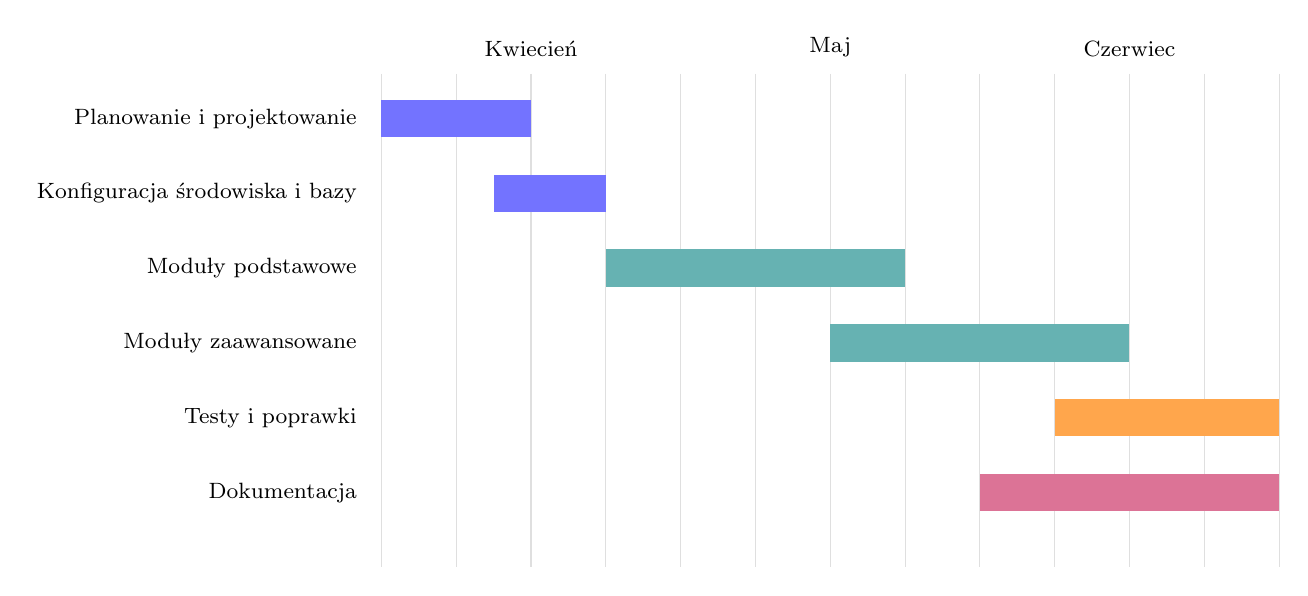
\begin{tikzpicture}[x=0.95cm, y=0.95cm, font=\footnotesize]
    % --- siatka tygodni ---
    \foreach \x in {0,1,2,3,4,5,6,7,8,9,10,11,12} {
      \draw[gray!25] (\x,0.3) -- (\x,-6.3);
    }
    % --- etykiety miesięcy ---
    \node[anchor=south] at (2,0.4)  {Kwiecień};
    \node[anchor=south] at (6,0.4)  {Maj};
    \node[anchor=south] at (10,0.4) {Czerwiec};
    % --- zadania: etykieta po lewej + pasek ---
    \node[anchor=east] at (-0.2,-0.3) {Planowanie i projektowanie};
    \fill[blue!55]  (0,-0.05) rectangle (2,-0.55);
    \node[anchor=east] at (-0.2,-1.3) {Konfiguracja środowiska i bazy};
    \fill[blue!55]  (1.5,-1.05) rectangle (3,-1.55);
    \node[anchor=east] at (-0.2,-2.3) {Moduły podstawowe};
    \fill[teal!60]  (3,-2.05) rectangle (7,-2.55);
    \node[anchor=east] at (-0.2,-3.3) {Moduły zaawansowane};
    \fill[teal!60]  (6,-3.05) rectangle (10,-3.55);
    \node[anchor=east] at (-0.2,-4.3) {Testy i poprawki};
    \fill[orange!70] (9,-4.05) rectangle (12,-4.55);
    \node[anchor=east] at (-0.2,-5.3) {Dokumentacja};
    \fill[purple!55] (8,-5.05) rectangle (12,-5.55);
  \end{tikzpicture}%
  }
  \caption{Diagram Gantta przedstawiający harmonogram realizacji projektu.\label{rys:gantt}}
\end{figure}

\section{Napotkane trudności w trakcie realizacji projektu}
\label{sec:trudnosci}

Podczas realizacji projektu napotkano kilka trudności, które wymagały dodatkowego czasu i uwagi:

\begin{itemize}
  \item \textbf{Mapowanie dziedziczenia na bazę danych} -odwzorowanie trzech hierarchii klas
        (użytkownicy, pytania, odpowiedzi) w bazie wymagało prawidłowej konfiguracji strategii
        Table-per-Hierarchy oraz dyskryminatorów w Entity Framework Core.

  \item \textbf{Reguły usuwania powiązanych danych} -konieczne było staranne dobranie reguł
        kaskadowego i ograniczającego usuwania, tak aby z jednej strony usunięcie testu czyściło
        powiązane dane, a z drugiej - edycja testu z istniejącymi rozwiązaniami nie naruszała
        oddanych już odpowiedzi uczniów.

  \item \textbf{Obsługa wielu podejść i wyboru najlepszego wyniku} -wymagała rozróżnienia między
        zapisem nowego podejścia a aktualizacją oceny istniejącego oraz spójnego liczenia wyników
        po stronie ucznia i nauczyciela.

  \item \textbf{Wykrywanie prób oszustwa} -konieczne było prawidłowe rozpoznawanie utraty fokusu
        okna oraz odróżnienie własnych okien dialogowych aplikacji od faktycznego przełączenia się
        użytkownika na inny program.
\end{itemize}

\section{Repozytorium i system kontroli wersji}
\label{sec:repozytorium}

Kod źródłowy projektu jest przechowywany i zarządzany za pomocą systemu kontroli wersji Git. Dostęp
do niego możliwy jest poprzez publiczne repozytorium w serwisie GitHub. Korzystanie z systemu
kontroli wersji pozwoliło na śledzenie wszystkich zmian w kodzie oraz zarządzanie kolejnymi wersjami
projektu.

\noindent Adres repozytorium projektu:\\
\url{https://github.com/MichalNocek/ProjektPO2}
